\documentclass[tikz, border=10mm]{standalone}


\newcommand{\track}[2]{%
  \begin{scope}[scale=#2]
 \draw [#1] plot [smooth cycle, tension=2] coordinates {(-0.5, 0) (-1, -1) (0,-1) (1,-1) (0.5, 0) (1, 1) (-1,1)};
\end{scope}}

\begin{document}
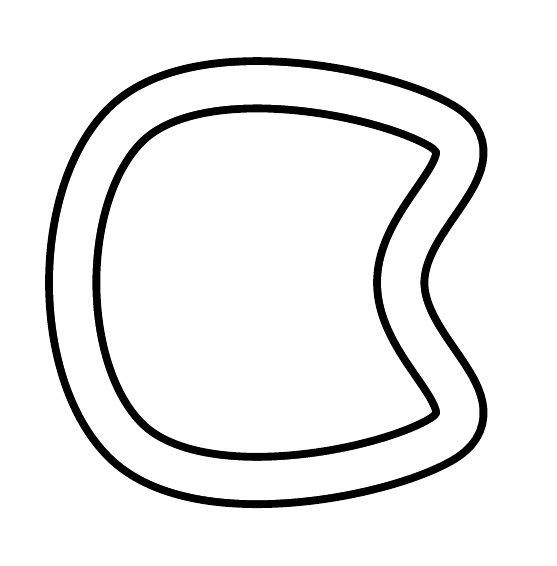
\begin{tikzpicture}
%\draw [black] plot [smooth cycle, tension=2] coordinates {(0, 0) (1, 0) (0.5, 0.5) (1,1) (0,1)};
%\track{black}{2}
%\track{red}{1.8}

\draw[double=white, double distance=5mm, line width=1mm] plot [smooth cycle, tension=0.8] coordinates {(-2, -2) (2, -2) (1.5, 0) (2, 2) (-2, 2)};

\end{tikzpicture}
\end{document}